\documentclass[12pt]{report} % formen af documentet
\usepackage[top=3cm, bottom=3cm, outer=2.5cm, inner=2.5cm, heightrounded]{geometry} %Margener
\linespread{1.2} %Linjeafstand
\usepackage[utf8]{inputenc} %Danske tegn
\usepackage [ danish ]{ babel} %danske overskrifter
\usepackage{graphicx} %til billeder
\usepackage{amsmath} % til formler
\usepackage{todonotes} %to do lister
\usepackage{tabulary} %for bedre at kunne håndtere tabeller

% pæn start på kapitler:
\usepackage[T1]{fontenc}
\usepackage{titlesec, color}
\definecolor{gray75}{gray}{0.75}
\newcommand{\hsp}{\hspace{20pt}}
\titleformat{\chapter}[hang]{\Huge\bfseries}{\thechapter\hsp\textcolor{gray75}{|}\hsp}{0pt}{\Huge\bfseries}
\setlength{\parindent}{0pt}


\section{Introduction}
Software is one of the essentials of the product, it is also one of the challenges for the business to exist. Since a business plan describes the fundamentals of the company and how it is going to make money, it is a critical section to describe the product, which will be done during this section. When there is a need of developing a software, the usual way would be to collect requirements from stakeholders. Currently the group is the only known stakeholder and therefore it is hard to create the usual procedure for the development. This would be a acquiring of requirements, create use cases, design a class diagram and keep it developed during the process. 

The development process is one of the key activities during the start up of the company. Therefore it is important to have focus of this specific process and making the choice of the right process. When in need of rapid development activities within the Scrum process would be attractive for the group, because it would implement the daily meeting which is used for sharing of problems and ideas for solving them. This requires an expert knowledge to become a useful process, which the group is eligible of.
\clearpage
\subsection{Current structure of the software system}
Figure \ref{ClassDiagram} shows the current state architecture of the software system. The system is far from complete and will grow during the development process. The modifications are hard to predict at this very moment, but this displays the main functions of the system and what focus areas there are within the development. 
\begin{figure}[h!]
\centering
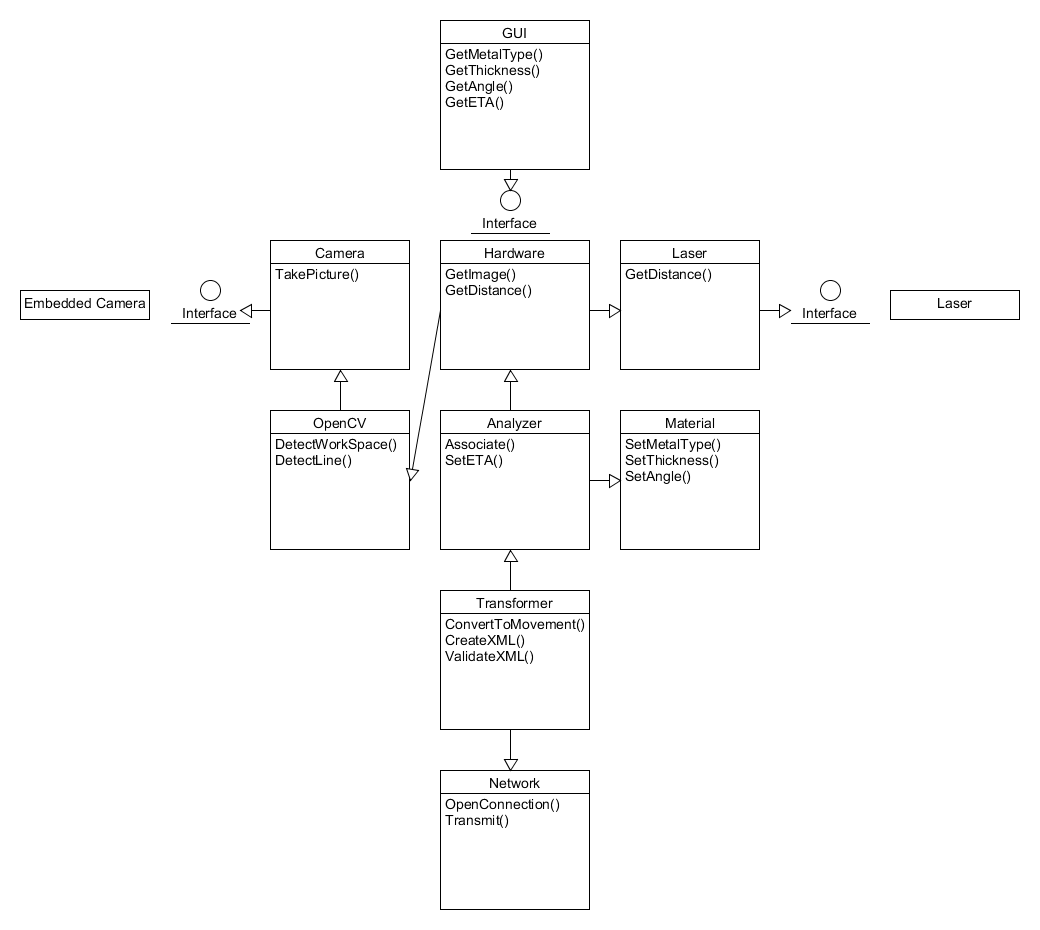
\includegraphics[width=0.7\textwidth]{graphics/ClassDiagram}
\caption{A simple class diagram for the prototype software system}
\label{ClassDiagram}
\end{figure}


\section{Product description}
The system is going to consist of multiple hardware parts, these parts will require interfaces to communicate with. Requirements is the word when it comes to designing software, it is what the stakeholders want. Requirements can be categorized, primary it is divided in functional and non-functional requirements. The non-functional are the passive requirements, these describe performance for instance. An example could be: "The AddOn should deliver movement coordinates for the robot within 2 minutes". In this section, the different interfaces will be described. 

\subsection{Hardware Interfaces}
Hardware is a major part of the product, these will require interfaces to communicate with the software system, since the default software for these hardware parts probably 'speaks' another language than the system. The usual way to approach this is by implementing adapter patterns, which includes a facade pattern. 

\begin{itemize}

\item Adapter pattern for the Laser Scanner output software
\item Network Interface between AddOn and a potential robot

\end{itemize}

Both the camera and laser scanner will come from different manufacturers, therefore there is no guarantee for the cooperation of their software. This is where an adapter pattern becomes usable within the system.

The network interface would have to fit specific standard within robotic interfaces. It is very dependant of the future partners and their choice of robotic interfaces.
  
\subsection{Software Interfaces}
Software interfaces are often used when it comes to facade parts of a system this helps making the objects unknown to other objects in the system. The purpose is the make a system with low coupling and high cohesion. Interfaces are also common to use when you have several objects or classes who needs the same method, so to lower the amount of 'copy + paste' code, you should implement interfaces instead. It is hard to identify methods that should be reinvented within the current prototype class diagram, which is why this subsection will not cover them. That is why the class diagrams will be updated during the development process of the software. 

\begin{itemize}

\item Facade pattern for the embedded camera
\item Facade pattern between user interface and logic layer

\end{itemize}

\subsection{User Interfaces}
User interfaces requires fundamental design to become useful for the end users. The design process often requires a huge amount of communication with the customers and stakeholders. User friendliness is the keyword within the design process. 

The AddOn will come with a sort of tablet for the end users to use. The tablet will provide a user interface for the end users to interact with. Different functionality is provided by this interface: 

\begin{itemize}

\item Selection of material to weld 
\item Define thickness of the object
\item Welding angle of the robot
\item Overview of different data, like ETA of the current welding, range of the laser scanner

\end{itemize}

This enables the end user to modify the welding process in a few steps. Importance of user friendliness is immense, since the time spent on modifying the process has to be compared to the time the user could spend somewhere else.

\section{Specific requirements}
Requirements are the fundamentals of specifying the distinct tasks to solve when creating a software system. Requirements can be divided into categories, which is done below:

\textbf{Functional Requirements:}
\begin{itemize}

\item The system should be able to communicate with the specified hardware
\item The system should be able to communicate with any welding robot, future partners suggest
\item The system should be able to take pictures with the embedded camera 
\item The system should be able to detect a line within the workspace of each picture provided by the embedded camera, by using OpenCV
\item The system should be able to create three dimensional coordinates based on inputs from a range scanner and a camera
\item The system should be able to convert movement-coordinates for the specific robot

\end{itemize}

\textbf{Non-functional Requirements:}

\begin{itemize}

\item The system should be able to create a moveable path for the robot within a tenth part of the time it takes to pickup the coordinates.
\item The precision of the laser should be within 0.05 cm
\item The precision of the robot movement should be within 0.05 cm of the coordinates

\end{itemize}

\subsection{Functions}

The system can be divided into three major functions, which handles the processing of detecting the place to weld, associate x,y an z coordinates and converts them into the movement program of a robot.

These actions can be divided into the following functions:

\begin{itemize}

\item DetectLine
\item Associate
\item ConvertToMovement

\end{itemize}

\textbf{DetectLine:}
By benefiting from the OpenCV library, this function is to detect the workspace area, by detecting the color marked by a worker, then detecting the line within.   

\textbf{Associate:}
This class has the task of gathering the two different data (camera coordinations and laser depth coordinations).

\textbf{ConvertToMovement:}
The final coordinates generated from the Associate class is being converted to an input which a robot can use. 

\subsection{Dependencies}
Using libraries can create dependencies within the system, mainly when a used library is dependant on other libraries. In this project, the OpenCV library will be in focus when extracting data of the line that the robot has to weld.   

\subsection{Database}
A database to log every entry is favourable for the end customer, but it is not a part of the AddOn and therefore not a part of the development process.

\subsection{System attributes}
System attributes describes the qualities of a system in short terms. Primary qualities of the system is going to be:

\begin{itemize}

\item Reliability
\item Precision
\item Maintainability
\item Adaptability

These attributes describes a system which is able to adapt to the customers robots, while being reliable and precise. 
\end{itemize}

\section{Design decisions}
Basically the system is set to follow the 3 layer structure. But as the system evolves it can be hard to predict whether this is going to chance or not. 

A factor which is common in the industrial is the request for real time actions within a network. This is not direct request, since a worker handles the robot and leaves it for its time to work. This mean that no special BUS networks are needed within the system and that a TCP protocol Ethernet network is a viable option. 

\section{Life cycle}

When the product has been developed and released it is far from complete, this is the reason for maintenance and repeating the working process of optimization and development. If the product is not updated, competitors and new ideas on the market is going to kill the business. Therefore it is important to repeat the actions described in the life cycle below:
\clearpage

\begin{figure}[ht]
\centering
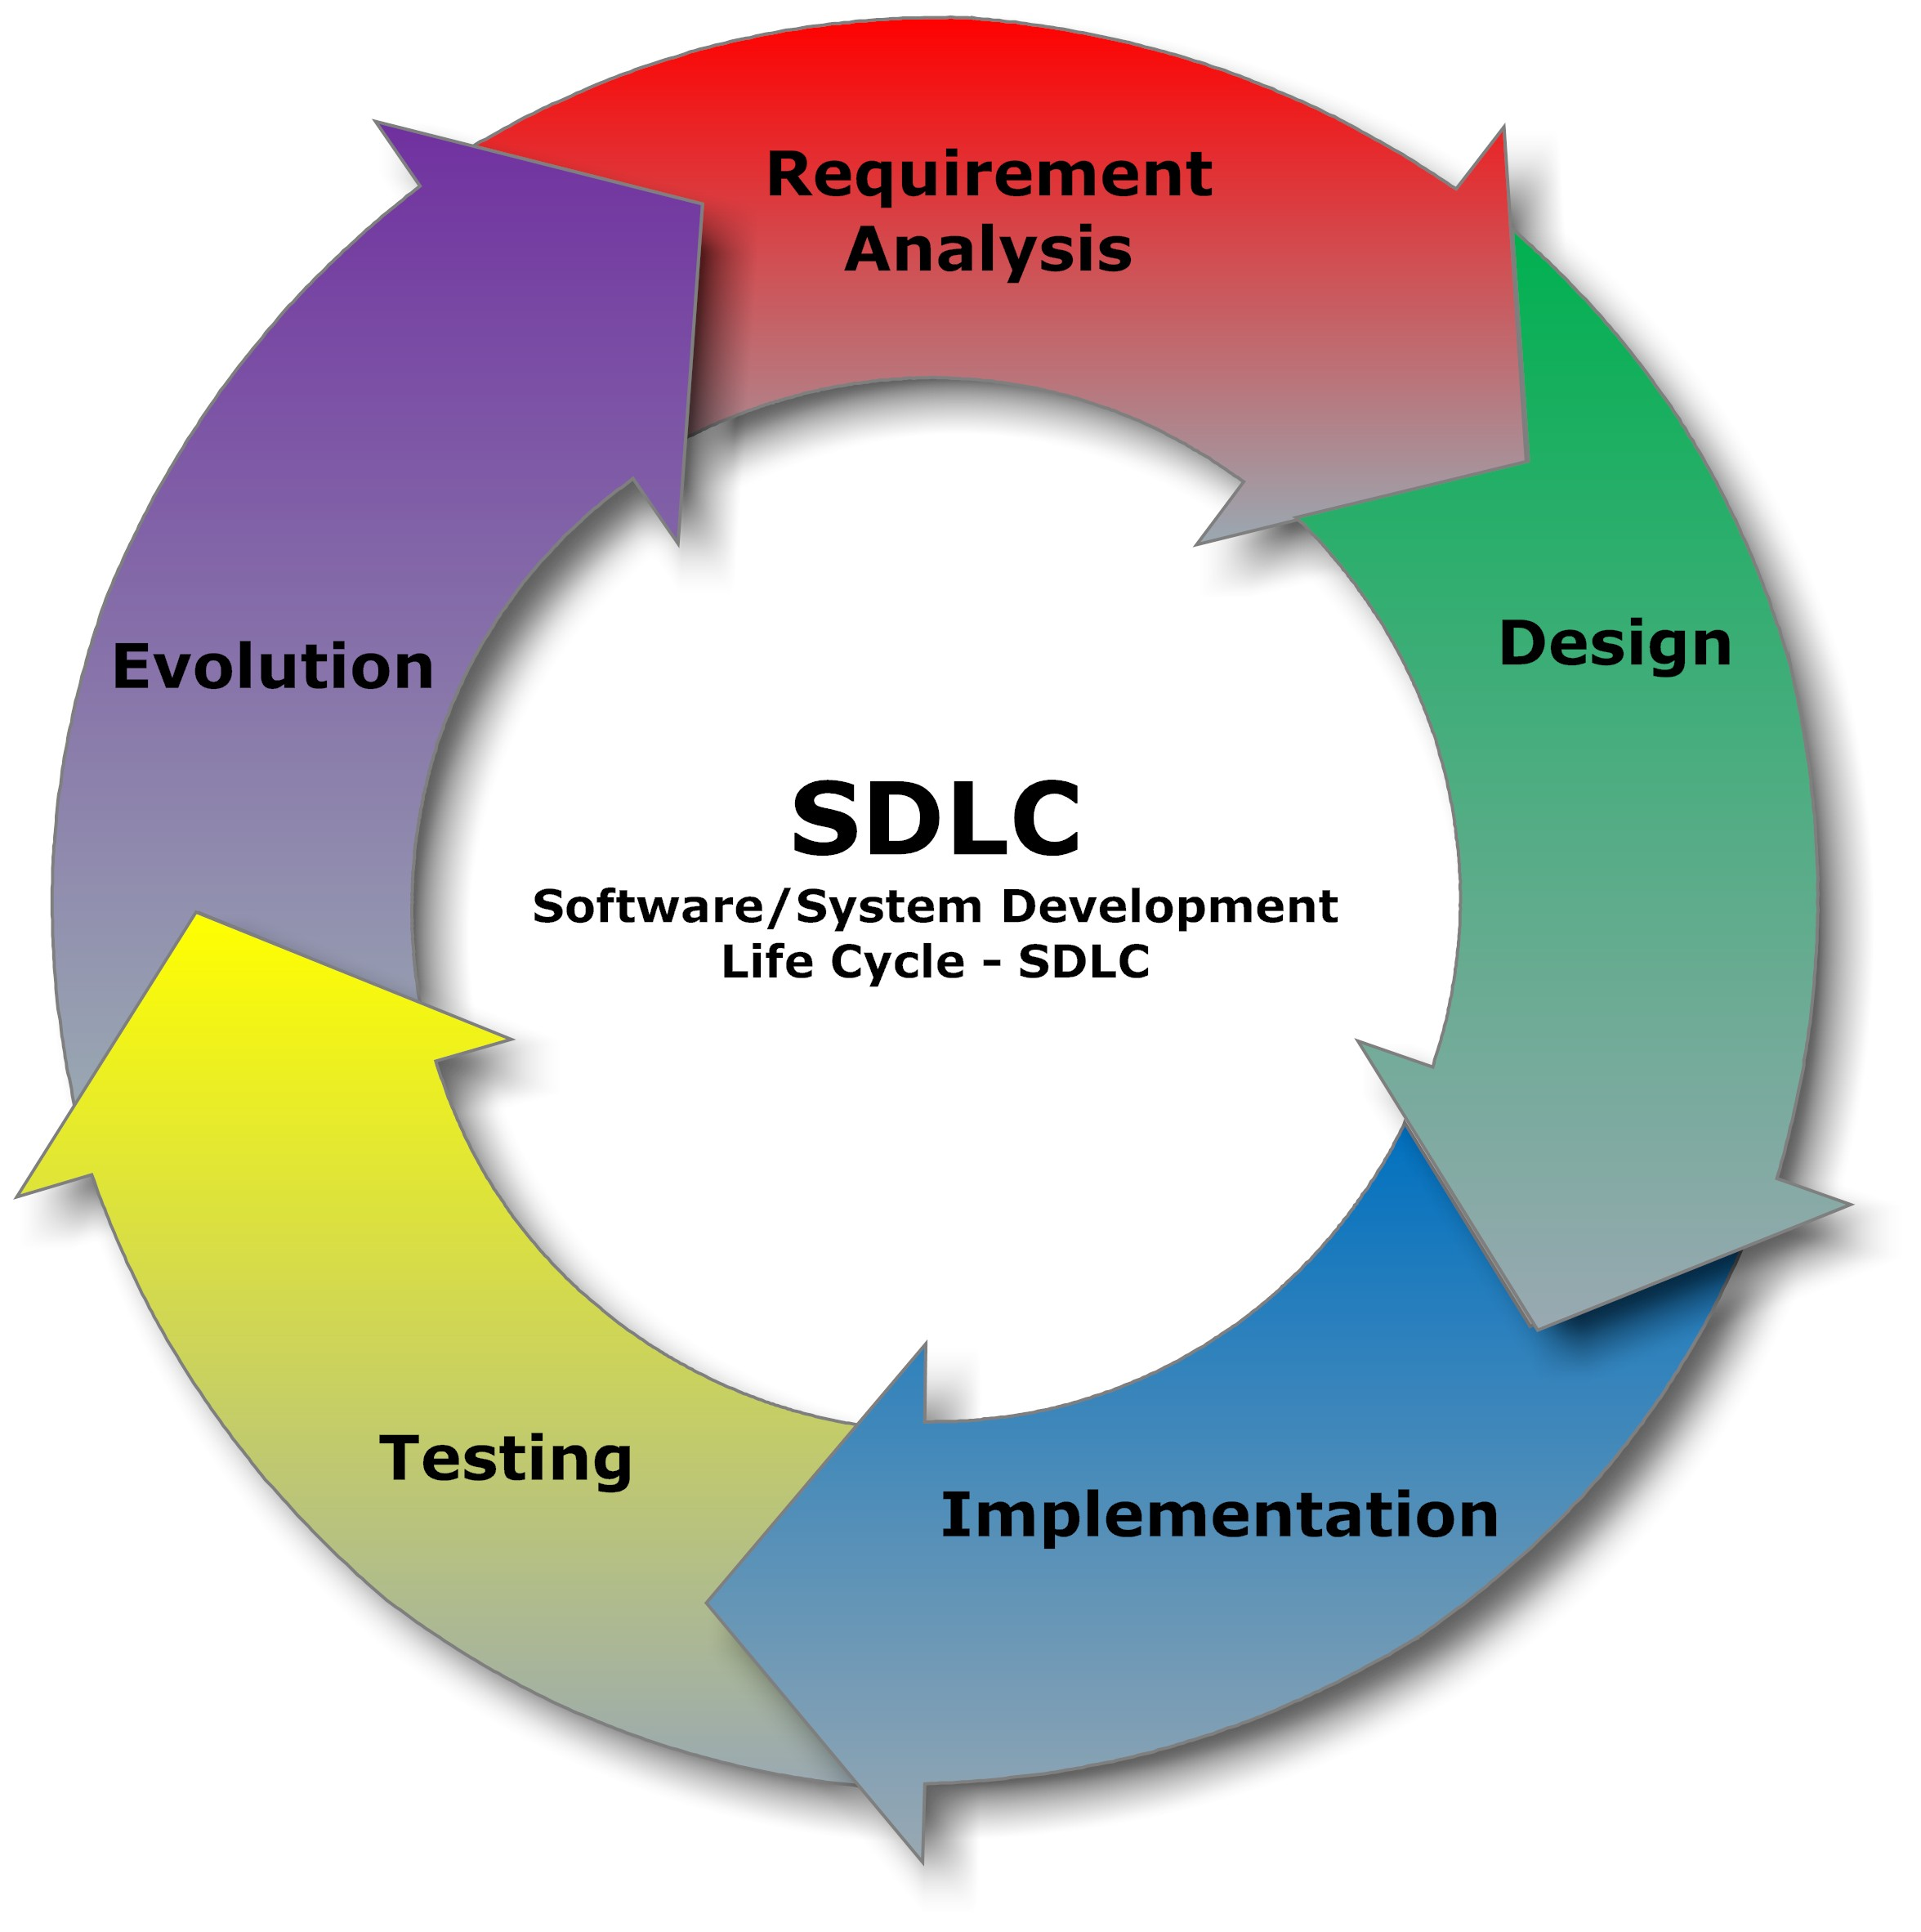
\includegraphics[width=0.5\textwidth]{graphics/Software_Development_Life_Cycle}
\caption{The life cycle describes the process of establishing and maintaining a system}
\label{SDLC}
\end{figure}
This process is not very detailed, because it is up to the developers and manage to choose a specific development process or a combination of them.

